% !TEX root = main.tex

\chapter{Méthode de simulation du tambour et assimilation de données}

Nous avons vu dans le chapitre précédent que l'assimilation dépendait de la définition d'un modèle et de son état. Dans le cas de la simulation de l'écoulement au sein du broyeur à boulets, il s'agit principalement de méthodes reposant des discrétisations sans maillage. C'est ce type de modélisaton qu'il faudra prendre en compte aussi lors de l'assimilation de données. Or, le caractère Lagrangien de la définition de l'état implique d'évaluer jusqu'à quel point les méthodes classiques d'assimilation peuvent être adaptée. En effet celles-ci se base sur des états dont la discrétisation ne varie pas au cours du temps. De plus, le fait que l'espace soit continu ou discret va également modifier la signification de l'état et sa capacité à être mis à jour.
Dans ce Chapitre, nous rappellerons en Section~\ref{sec:simu_broyeur} les principales méthodes utilisées aujourd'hui pour simuler l'écoulement au sein du broyeur à boulet. En constatant la prédominance des méthodes sans maillage, nous reprendrons les principales familles de formulation particulaire en particulier en considérant en Section~\ref{sec:part_discret} les méthodes utilisant un milieu discret et en Section~\ref{sec:part_cont} un milieu continu. Nous évoquerons les sigularités et limites à l'adaptation des méthodes d'assimilation de données et présenterons les travaux actuels dans la littérature. De plus, nous présenterons la méthode vortex comme une méthode particulaire modèle pour la suite du manuscrit.

\section{Ecoulement d'un milieu granulaire}

La simulation du broyeur repose sur la représentation de l'écoulement d'un milieu granulaire. Si les écoulements granulaires sont très présents dans la nature et dans l'industrie, du fait de la nature discrète du milieu, ils sont bien moins comprise que l'écoulement d'un liquide qui se base sur les équations de Navier-Stokes.
L'écoulement granulaire va se distinguer par trois types de régime que l'on assimile généralement au trois état de la matière: solide où où le mouvement des particules est lent et le comportement est presque statique, une couche semblable à un liquide dans laquelle les grains s'écoulent avec une certaine inertie, et une zone semblable à un gaz où les particules se déplacent à des vitesses plus élevées de manière chaotique. Ils interviennents simultanément dans l'écoulement. Ce qui complexifie sa caractérisation rhéologique.

\begin{figure}
    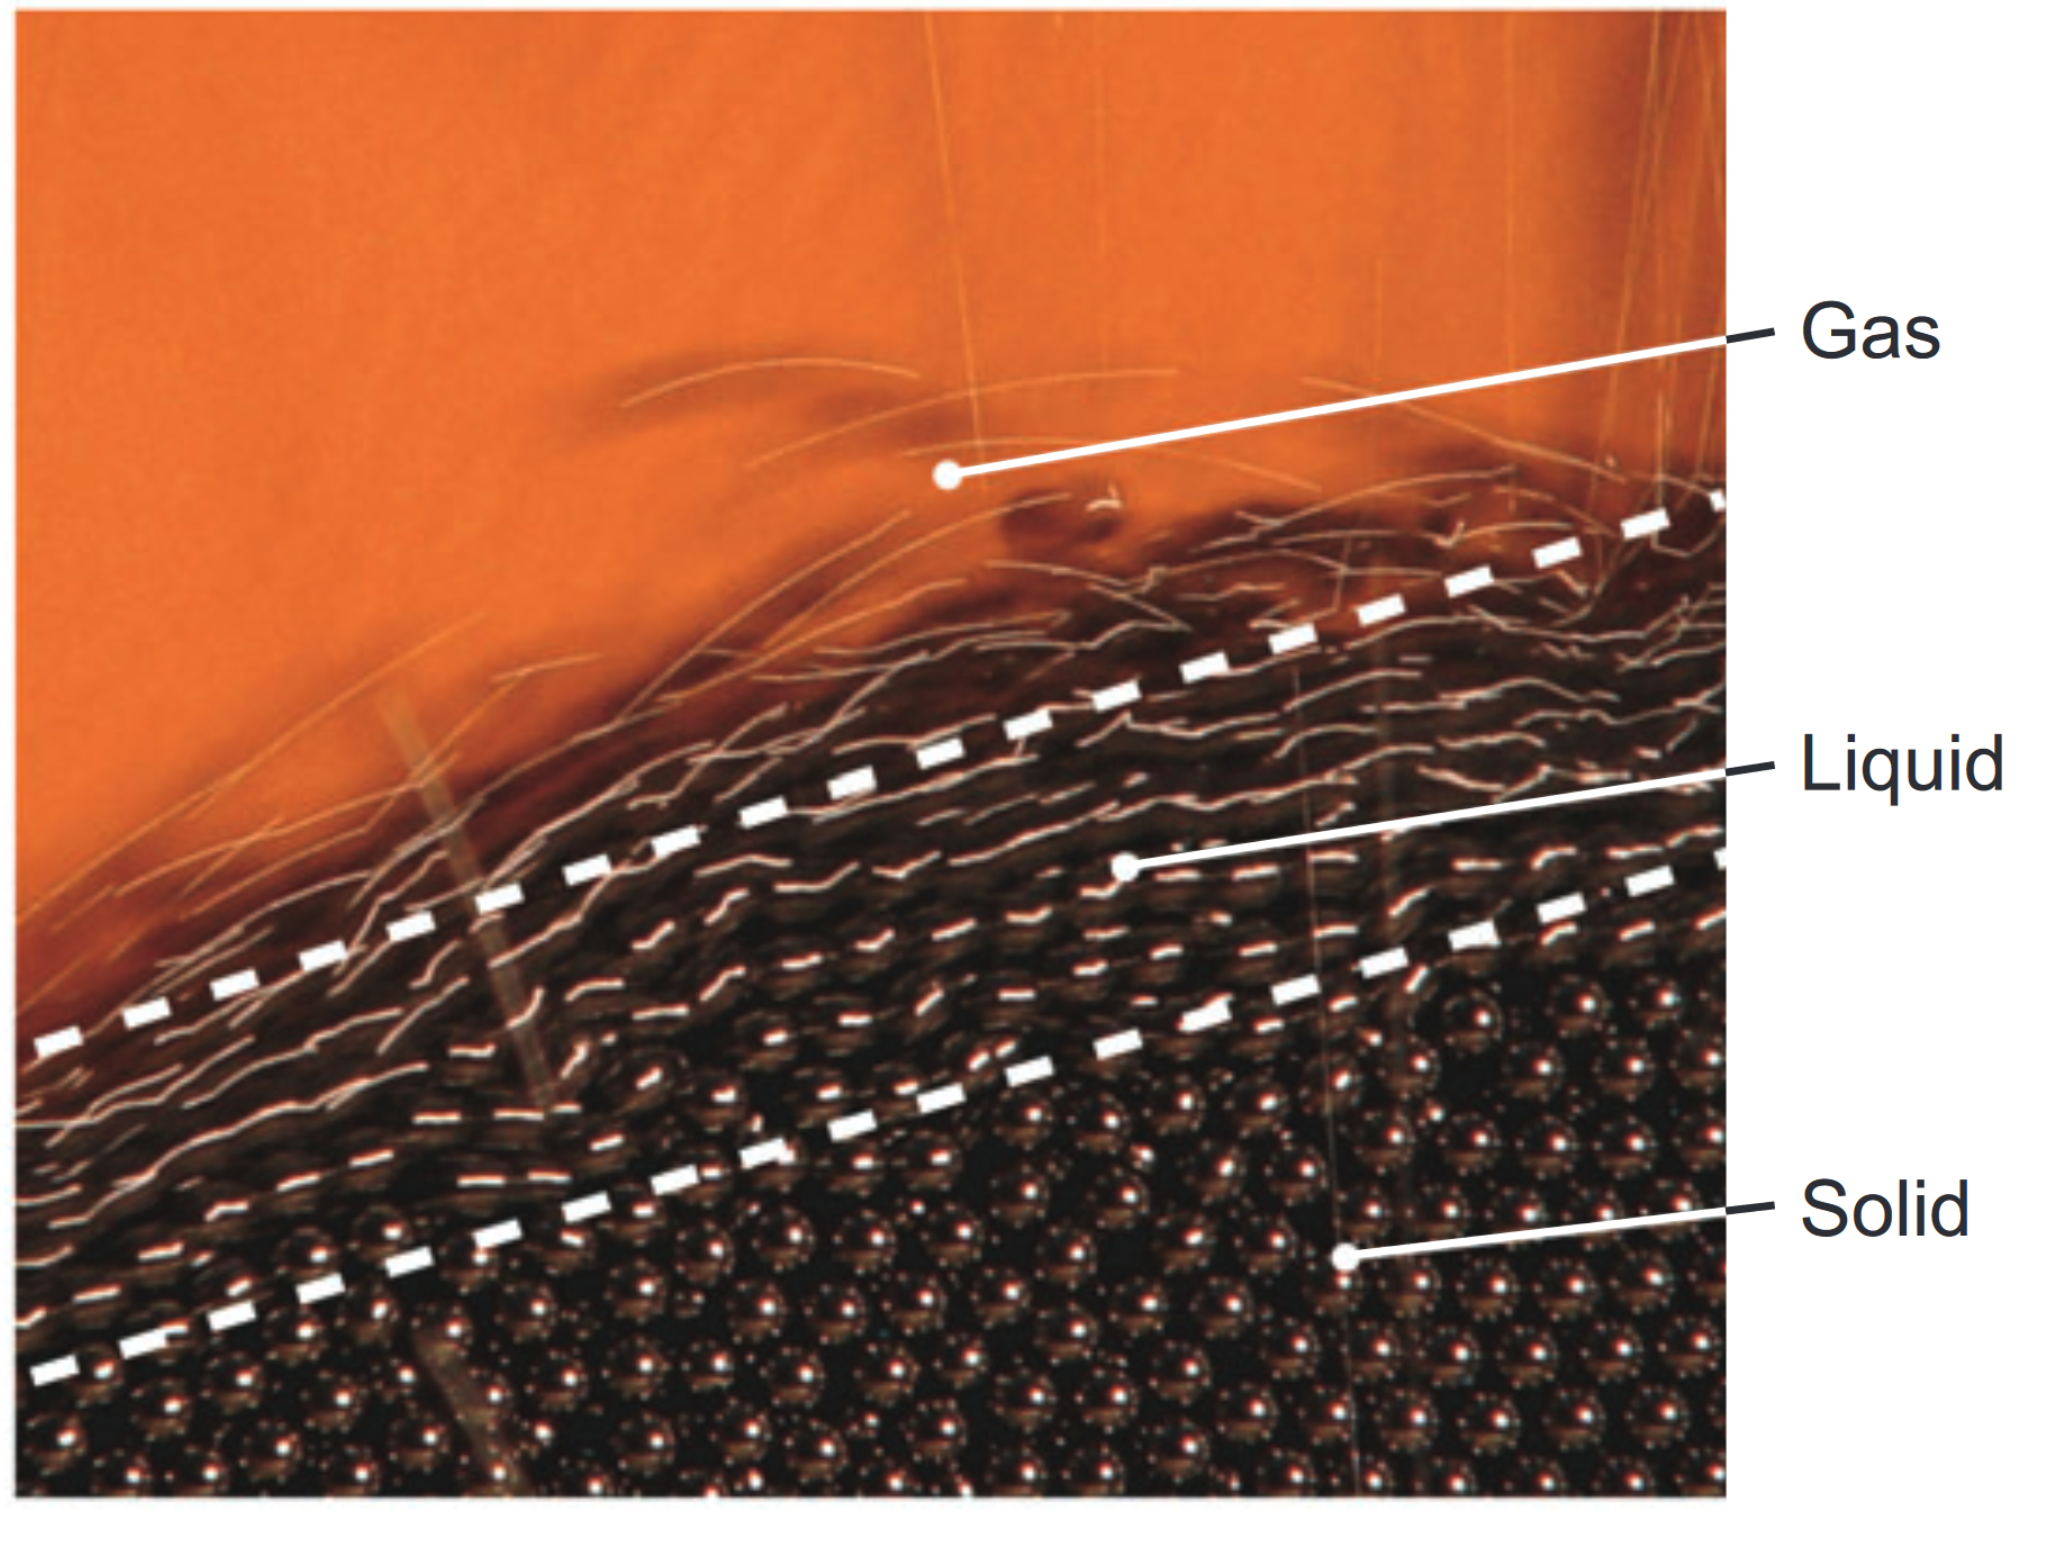
\includegraphics[width=\textwidth]{three_regimes.png}
    \caption{Image de billes d'acier s'écoulant d'un tas. Trois phases de l'écoulement granulaire, se comportant comme un gaz, un liquide ou un solide, peuvent être identifiées.~\cite{forterre_flows_2008}}
\end{figure}

Les régimes solides interviennent

Les travaux récents convergent vers une loi de comportement viscoplastique pour modéliser les milieux granulaires défini sous le nom de loi $\mu(I)$ \cite{gdr_midi_dense_2004,jop_constitutive_2006} ce qui a permis de développer des simulation du tambour en rotation~\cite{Cortet_2009} et montre une bonne correspondance pour le cas d'écoulement avec surface libre \cite{chou_cross-sectional_2009}.
Toutefois, cette loi trouve certaines limites dans le cas d'écoulement confiné où le coefficient de tassement change et où le mouvement de chaque grain entraîne des modifications significatives dans les chaînes de force. Si la prédiction est bonne au niveau des bords, elle reste toutefois insufisante au niveau des parois \cite{Rognon_Miller_Metzger_Einav_2015}. De plus, elle ne permet pas de prendre en compte les régimes cinétiques, c'est à dire le régime gaz. Ainsi, le développement de nouvelles loi rhéologique est un sujet de recherche constant.

\section{Simulation du tambour}\label{sec:simu_broyeur}

Dans le tambour en rotation l'ensemble des trois zones d'écoulement sont présentes. Divers régimes d'écoulement tel que : glissement, ballotement, éboulement, roulement, en cascade, cataracte,  centrifuge~\cite{MELLMANN2001251}.
Ces différents régimes déterminent la qualité du mélange, du broyage. C'est le régime en cascade qui est nécessaire pour la réduction de taille de grain dans le broyeur à boulets. C'est dans ce régime que la surface libre prend la forme caractéristique d'un \textit{S}.

Outre la difficulté dans la définition de la loi de comportement, c'est aussi le type de simulation qui est complexe dans le cas de la simulation du tambour. En effet, ce problème présente un cas d'écoulement en grande transformation, avec une surface libre et nécessite de tenir compte des interactions avec une paroi mobile voir les corps broyants.

% APPROCHE DISCRETE
Avantages :
Etude du mélange : Représente très bien les différents régimes d’écoulement, de ségrégation
Prise en compte d’une grande variété de géométrie de particule
Spectre de collision : permet une estimation de la fonction de rupture (source ?)

Inconvénients :
Très couteux (en particulier la détection des contacts)
Réalisation de simulations à grande échelle
Difficultés de mise à jour des états en fonction des observations

% APPROCHE CONTINUE
%% CFD / FEM
Avantages
Adapté à la simulation d’écoulement à grande échelle
Inconvénients
Définition de la loi de comportement complexe dépendante du régime de vitesse
Lois de comportement en mécanique des sols : Mohr-Coulomb : faible vitesses
Modèles rhéologiques : $\mu(I)$ vitesses intermédiaires
Modèles basés sur la cinétique des gaz : hautes vitesses

%% MPM 
Avantages
Prise en compte des problèmes de grandes transformations : pas de distorsion de maillage ;
Conservation de la masse et de la quantité de mouvement par construction (et le moment angulaire avec la méthode APIC) ;
Deux représentations possibles de l’état du système ;
Prise en compte d’un mélange de différents matériaux ainsi qu’une surface libre ;
Implémentations parallèles existantes sur GPU/CPU.

Inconvénients
Moins efficace que la méthode FEM : nécessite de recalculer les fonctions d’interpolation grille/particules

Appliquée au cas des écoulements granulaires par Soundararajan 2015

Appliqué au problème du tambour en rotation dans deux articles :

Zuo et al. « Numerical Simulation of Granular Mixing in a Rotary Drum Using a Generalized Interpolation Material Point Method ». Asia-Paci1c Journal of Chemical
Engineering (2020).

Chandra et al. « Nonconforming Dirichlet Boundary Conditions in Implicit Material Point Method by Means of Penalty Augmentation ». Acta Geotechnica (2021).

% Avec les approches continues l'intérieur du tambour d'un mélangeur-broyeur est conceptualisé comme un milieu continu, adoptant une perspective macroscopique. La réponse du milieu est alors représenté par une loi de comportement mécanique telle que la loi de Drucker-Prager. Cela contraste avec la méthode des éléments discrets (DEM), qui se concentrent sur les interactions particule-par-particule.

% Cette approche hybride permet à la MPM de capturer efficacement les déformations importantes, les ruptures, et d'autres comportements complexes du milieu qui sont fréquents dans les opérations de mélange et de broyage. En revanche, la description fine du phénomène proposée par la DEM n'est plus disponible.

% En termes de temps de calculs, la MPM est plus efficace que la DEM.

\section{Méthodes sans maillage discrètes}~\label{sec:part_discret}

url         = {https://hal.science/hal-01824750},
Les méthodes sans maillage discrètes traitent les particules comme des objets solides indépendants. Ces entités physiques sont caractérisées par leur géométries, ainsi que par des propriétés intrasèques qu'elles conservent tout au loin de la simulation. Les particules interagissent entre elles au travers de lois de contact, de frottement et de cohésion. L'objectif est de déterminer la trajectoire des particules. Parmis ces méthodes, on peut mentionner la méthode des éléments discrets (DEM)~\cite{radjai:hal-00691805} et la méthode de dynamique des contacts (CD)~\cite{moreau:hal-01824750}.


% UTILISER PARTIE LHASSAN

\subsection{Méthode des éléments discrets (DEM)}
Référence dans la simulation des écoulements granulaires.
Appliquée aux broyeurs dès 1992 par Mishra and Rajamani d’abord en 2D puis en 3D
Bonne confrontation aux acquisitions expérimentales
Permet d’obtenir des informations de champs de vitesse, la surface libre, la distribution des collisions, …




La méthode consiste à considérer le mouvement d'un ensemble de $N$ grains composant le milieu. Celui-ci est décrit par l'équation de la dynamique qui peut s'écrire sous la forme

\begin{equation*}
    \left\{
    \begin{aligned}
         & m_{i} \frac{ d^{2}\vec{r}_i }{dt^2}=\vec{f}_{i},\; i=1\ldots N      \\
         & I_{i} \frac{d \vec{\omega}_{i}}{dt}=\vec{\Gamma}_{i},\; i=1\ldots N
    \end{aligned}
    \right.
\end{equation*}où $`N`$ est le nombre de grains, $`m_{i}`$ est la masse, $`I_i`$ est le moment d'inertie, $`\vec{r}_{i}`$ est la position, $`\vec{\omega_{i}}`$ est la rotation, $`\vec{f}_{i}`$ est la force exercée sur le grain considéré et $`\vec{\Gamma_{i}}`$ le moment associé à la force $`\vec{f}_{i}`$.

La force $`\vec{f}_{i}`$ peut être décomposée de la manière suivante

\begin{equation*}
    \vec{f}_{i}=\underset{{\scriptstyle j\neq i}}{\sum}\vec{f}^{c}_{ij}+\vec{f}_{ext}
\end{equation*}

où $\underset{{\scriptstyle j\neq i}}{\sum}\vec{f}^{c}_{ij}$ représente les forces de contact qui s'exercent à la surface de la particule $i$ et les forces externes $`\vec{f}_{ext}`$ sont celles appliquées au centre de la particule $`i`$ (par exemple la force de gravité).

Les forces de contact sont décrite par des loi de contact entre les grains ainsi qu'entre les grains et la paroi. Dans le cas élastique, la modèle de Hertz est adapté pour décrire l'intéraction normale. Le modèle Hertz-Mindlin permet de déterminer les interactions tangentielles élastiques. Ces loi sont fonctions de l'interpénétration inter-particule et de la vitesse relative interpaticules. Par exemple, dans le cas de particules sphérique l'interpénétration est défini comme $\delta_{ij} = \norm{\bm x_i - \bm x_j} - (R_i - R_j)$ où $x$  est la position et $R$ le rayon d'une particule.

La force de contact tend à pénaliser l'interpénétration via des coefficients de raideur $k$ et d'amortissement $\gamma$ qui dépendent des propriétés mécaniques des grains de de la paroi. Il existe plusieurs algorithme pour résoudre numériquement les équations de la dynamique. Le plus utilisé est l'algorithme de Verlet en vitesse.


La méthode des éléments discrets (DEM, pour \textit{Discrete Element Method}) est une technique de simulation numérique utilisée pour étudier le comportement des systèmes de particules, tels que lors du mélange broyage à l'intérieur du broyeur à boulets. Cette approche est particulièrement pertinente pour modéliser les interactions complexes entre les particules dans ces systèmes, où la dynamique individuelle de chaque particule peut avoir un impact significatif sur le processus global.

Dans un mélangeur-broyeur, les particules interagissent entre elles, avec les parois du broyeur, et avec le corps broyant. La DEM modélise chaque particule individuellement, en tenant compte de ses propriétés physiques telles que la taille, la forme, la masse, la rigidité, et le modèle de fragmentation. Les interactions incluent les forces de contact, les forces de frottement, et les forces de cohésion.

Le processus de simulation DEM dans un mélangeur-broyeur commence par la définition des propriétés des particules et des conditions initiales du système. Le mouvement de chaque particule est ensuite calculé en résolvant les équations de Newton pour le mouvement et la rotation. Ces calculs tiennent compte des forces et des moments résultant des collisions et des interactions entre particules, ainsi que de l'interaction des particules avec les parois du broyeur.

L'un des principaux avantages de la DEM est sa capacité à fournir des informations détaillées sur le mélange et le broyage des particules à l'échelle microscopique. Elle permet d'analyser comment les variations dans la configuration des particules, la vitesse de rotation du broyeur, et d'autres paramètres opérationnels influencent l'efficacité du broyage et l'homogénéité du mélange.

Cependant, l'utilisation de la DEM pour la simulation de mélangeurs-broyeurs peut être exigeante en termes de ressources informatiques, en particulier pour les systèmes avec un grand nombre de particules.

\subsection{DEM et assimilation de données}

L'assimilation de données, lorsqu'appliquée à des systèmes simulés par la méthode des éléments discrets (DEM), se heurte à plusieurs limites importantes présentées ci-dessous.

% \subsubsection{Limites de la DEM avec les méthodes variationnelles}
Dans le cadre des méthodes variationnelles d'assimilation de données, telles que 3D-Var, le principal défi est la grande dimensionnalité du problème d'optimisation.
En effet, La DEM simule le comportement de chaque particule individuellement. Cela signifie que l'état du système comprend les variables cinématique de chacune d'elles : position, la vitesse, accélération mais aussi la position angulaire, la vitesse angulaire et l'accélération angulaire ou la densité de chaque particule. Pour un système avec des milliers voire des millions de particules, cela conduit à un problème d'optimisation de très grande dimension.

De plus, il existe un nombre extrêmement élevé de contraintes, notamment l'interdiction de l'interpénétration des particules. Ces contraintes doivent être prises en compte pour assurer que la solution d'optimisation soit physiquement admissible.

L'application des méthodes 3D-Var et 4D-Var est donc trop exigeante d'un point de vue des temps de calcul.

De plus, les filtres variationnels corrigeant des erreurs d'intensité selon des normes euclidiennes, la variation selon les positions des observations ne sera pas linéaire.

Ainsi, la définition d'un état de particules discrètes implique de résoudre un problème d'optimisation non-linéaire de grande dimension.
% \subsubsection{Limites de la DEM avec EnKF}
Pour l'EnKF, l'état estimé du système est une combinaison linéaire des états prédits par les différents membres de l'ensemble. Cependant, dans le contexte de la DEM, cette combinaison linéaire des états n'est pas nécessairement physiquement admissible. Par exemple, elle pourrait conduire à des situations où les particules s'interpénètrent ou violent d'autres lois physiques.
En d'autres terme, la mise à jour ne peut être réalisé que via le solveur lui-même capable de vérifier des contraintes de non interpénétrabilité mais ne peut être réalisé directement.

Un autre problème avec l'EnKF dans le contexte de la DEM est la difficulté de faire correspondre les particules entre les différents membres de l'ensemble. Même si initialement chaque membre possèdait la même configuration particulaire mais avec des propriétés différentes, chaque particule a sa propre trajectoire unique en cohérence avec les intéractions dans son voisinage. Aligner ces trajectoires à travers les différents membres de l'ensemble pour une assimilation de données cohérente est un défi complexe. Cette difficulté est exacerbée par le nombre élevé de particules et par la nature dynamique et chaotique de leurs interactions.

Dans le cas pus général où les membres n'aurait pas le membre de particule la correspondance des états est d'autant plus complexe.

Ainsi, le caractère discret de la méthode DEM rend l'assimilation par EnKF à la fois complexe par :

\begin{itemize}
    \item une définition de l'état et de ses statistiques non univoque ;
    \item la construction du gain de Kalman d'Ensemble ;
    \item la contrainte d'interpénétration non respecté lors de la mise à jour.
\end{itemize}

\section{Méthodes particulaires continues}\label{sec:part_cont}
Nous envisageons des méthodes par particules pour résoudre des problèmes continus en mécanique des fluides ou des solides. Cela inclut des méthodes telles que l'hydrodynamique par particules lissées (SPH) \cite{lucy_1977,gingold_monaghan_sph_1977} et la méthode des vortex (VM) \cite{cottet_vortex_2000}, et s'étend à d'autres méthodes comme la méthode des points de matériau (MPM) \cite{sulsky_particle_1994}. Elles partagent toutes de décomposer cette fois le domaine en un ensemble $\mathcal{P}$ de particules qui suivent la dynamique du problème. Ainsi, la discrétisation suit la transformation appliquée au milieu en transportant des quantités attachées à chaque particule. Elles sont en cela des méthodes Lagrangienne.

\subsubsection{Discrétisation par particules}

La solution représentée par le jeu de particule est obtenue grâce à deux éléments: une appproximation grâce à un noyau de lissage et l'approximation particulaire d'un opérateur intégral. Si la représentation de la solution peut évoluer suivant la méthode (en particulier avec la méthode MPM), la solution peut toujours être exprimé de cette manière suivant le choix du noyau.

Tout champ relativement régulier $\bm{u}$ sur $\Omega$ peut être écrit grâce à la propriété de filtrage de Dirac

\begin{equation*}
    \bm{u}(\bm{z}) = \int_{\Omega} \bm{u}(\bm{z'}) \delta(\bm{z'} - \bm{z})  d\bm{z'},
\end{equation*}avec $\delta$ la distribution de Dirac.

Une fonction de noyau $\phi_\varepsilon$ est introduite pour obtenir une estimation moyenne $\langle \bm{u} \rangle$ de $\bm{u}$ telle que

\begin{equation*}
    \langle \bm{u}(\bm{z}) \rangle = \int_{\Omega} \bm{u}(\bm{z'}) \phi_\varepsilon(\bm{z}-\bm{z'}) d\bm{z},
\end{equation*}où $\varepsilon$ est la longueur de lissage. Le noyau lisse doit au moins respecter les propriétés suivantes

\begin{eqnarray*}
    && \int_{\Omega} \phi_\varepsilon(\bm{z}) d\bm{z} = 1,      \\
    && \phi_\varepsilon(\bm{z}) \to \delta(z), \quad \varepsilon \to 0, \\
    && \phi_\varepsilon(\bm{z}) \in C^k,  \quad k \geq 1,
\end{eqnarray*} où les deux premières propriétés sont des propriétés résiduelles de la distribution de Dirac et la dernière est une exigence de différentiabilité nécessaire pour approcher les opérateurs différentielles.

La fonction moyenne $\langle \bm{u} \rangle$ est ensuite utilisée pour approximer la fonction d'origine.

Dans un second temps, le domaine d'origine $\Omega$ est subdivisé avec $N_p$ sous-domaines $\Omega_p$ associés à une particule Lagrangienne à l'emplacement $z_p \in \Omega_p$. Nous notons $V_p$ le volume de $\Omega_p$. Cette discrétisation est ensuite utilisée pour approximer la fonction moyenne de telle sorte que

\begin{eqnarray*}~\label{eq:part_approx}
    \langle \bm{u}(\bm{z}) \rangle &=& \sum_p \int_{\Omega_p} \bm{u}(\bm{z'}) \phi_\varepsilon(\bm{z}-\bm{z'}) d\bm{z'} \\
    &\approx& \sum_p \bm{u}(\bm{z}_p) V_p \phi_\varepsilon (\bm{z}-\bm{z}_p) \\
    &\approx& \sum_p \bm{U}_p \phi_\varepsilon (\bm{z}-\bm{z}_p).
\end{eqnarray*}

Ainsi, toute fonction définie sur une discrétisation par particules est définie par un ensemble de positions de particules $\bm{z}_p$ associées à une valeur de particule $\bm{U}_p = \bm{u}(z_p) V_p$ et un noyau lisse $\phi_\varepsilon$.

Sur la base de cette discrétisation, l'opérateur différentiel peut être dérivé à travers cette formulation.

Tout comme le champ $\bm u$, la même interpolation peut être appliquée pour obtenir

\begin{equation*}
    \nabla \bm{u}(\bm{z}) = \sum_p \bm{U}_p \nabla \phi_\varepsilon (\bm{z}-\bm{z}_p).
\end{equation*}

Ils existent toutefois une grande variété de formule pour approximer l'opérateur gradient. Dans ces cas, ce sont les propriétés de conservation associées au champ qui sont privilégiées.
Généralement, un terme additionnel est introduit lorsque le champ est évalué à la position d'une particule $q$ tel que

\begin{equation*}
    \nabla \bm{u}(\bm{z}_p) = \sum_q (\bm{U}_q - \bm{U}_p) \nabla \phi_\varepsilon (\bm{z_q}-\bm{z}_p)
\end{equation*}, où $\sum_q \bm{U}_p \nabla \phi_\varepsilon (\bm{z_q}-\bm{z}_p)$ est nul par propriété de localisation du noyau $\phi_\varepsilon$.

% Finalement dire qu'il y a donc des équations qui permettent de définir l'évolution des intensités ainsi que des positions.

\subsubsection{Exemple de fonctions de noyau}

Plusieurs noyaux ont été utilisés en fonction de la méthode. La formulation originale de la MPM n'utilisait pas de noyau de substitution et écrivait la densité comme suit

\begin{equation*}
    \bm{u}(\bm{z}) = \sum_p \bm{U}_p \phi_\varepsilon (\bm{z}-\bm{z}_p)
\end{equation*}

Et la résolution est basée sur une projection sur une grille de fond associée à certaines fonctions de forme \cite{sulsky_particle_1994}.

La méthode GIMP est une formulation différente qui utilise la fonction de Heaviside \cite{bardenhagen_generalized_2004} et associe donc un volume autour de chaque particule

\begin{equation*}
    M_1(r) = \frac{\alpha}{\varepsilon}\left\{\begin{aligned}
         & 1; & r \leq \varepsilon \\
         & 0; & \text{sinon}
    \end{aligned}
    \right.
\end{equation*}où $r = \norm{\bm{z}}_2$.

Cette méthode a été introduite pour éviter le problème de passage de cellule lorsque une particule se déplace d'une cellule à une autre à travers la grille de fond.

Dans la méthode SPH, comme son nom l'indique, un noyau lisse est associé pour approximer la solution. Théoriquement, il pourrait s'agir de la fonction de noyau gaussien

\begin{equation*}
    \phi_g(r) = \frac{1}{{(\pi \varepsilon^2)}^{d/2}} \exp(-r^2/\varepsilon^2)
\end{equation*}.

Ce noyau est infiniment différentiable mais défini sur un support non compact. En pratique, nous utilisons une coupure pour supprimer les valeurs négligeables pour une grande distance par rapport à une particule.

D'autres noyaux, basés sur des fonctions B-Spline pour travailler sur un support compact. Ces fonctions sont également positives, ce qui est une exigence pour certains champs comme la densité.

Par exemple, le B-spline quadratique, que nous appelons $M_3$, est défini avec
\begin{equation}~\label{quadratic_kernel}
    M_3(r) = \frac{\alpha}{\varepsilon^d}\left\{ \begin{aligned}
         & \frac{3}{4} - |q|^2                            & 0 \leq           & |q| < \frac{1}{2} \\
         & \frac{1}{2} {\left(\frac{3}{2} - |q|\right)}^2 & \frac{1}{2} \leq & |q| < \frac{3}{2} \\
         & 0                                              & \frac{3}{2} \leq & |q|
    \end{aligned}
    \right.
\end{equation}avec $r = \norm{z}_2 $ et $q = r / \varepsilon$ et $\alpha$ la condition de normalisation et $d$ la dimension spatiale.

Ce noyau garantit la continuité $C^1$.
Le noyau cubique est un autre noyau B-Spline qui est
\begin{eqnarray}~\label{cubic_kernel}
    M_4(r) &=&  \frac{\alpha}{\varepsilon^d} \left\{ \begin{aligned}
         & \frac{1}{6}{(-|q|+2)}^3 - \frac{4}{6}{(-|q|+1)}^3 & 0 \leq      & |q| \leq  1 & \\
         & \frac{1}{6}{(- |q|+2)}^3                          & 1      \leq & |q| \leq 2  & \\
         & 0                                                 & 2 \leq      & |q|
    \end{aligned}
    \right.
\end{eqnarray}

Dans ce dernier cas, le facteur de normalisation $\alpha$ est

\begin{equation*}
    \alpha = \left\{ \begin{aligned}
         & 1;    \quad      & 1\text{ d} \\
         & 30/14 \pi; \quad & 2\text{ d} \\
         & 3/ 2\pi; \quad   & 3\text{ d}
    \end{aligned}
    \right.
\end{equation*}

Notez que ces noyaux ont été définis avec la coordonnée radiale $r$. Une autre possibilité serait de définir le noyau multidimensionnel comme le produit tensoriel du noyau 1D

\subsection{Distribution particulaire admissible}

Les méthodes sans maillage sont ici des méthodes d'appoximation de champs continus. Ces discrétisations doivent ainsi vérifier un certain nombre de critère pour être conforme à la solution. Il s'agit en particulier de donner ici des critères de régularité pour définir si une méthode d'interpolation sans maillage est valide. On trouvera des détailes supplémentaires dans le livre~\cite{s_li_meshfree_2004} en section 4.

On rappelle tout d'abord ce qu'est le support d'une particule $p$. Chaque particule est associée à une fonction d'interpolation $\phi_\varepsilon(\bm{z})$. Le support compact est donc

\begin{equation*}
    S_p = \{\bx \mid \| \phi_\varepsilon \bx - \bx_p \| > 0\} \cap \Omega,
\end{equation*}

On définit également $\rho_p$ le rayon du support compact comme
\begin{equation*}
    \rho_p =  \max \{\| \bx - \bx_p \| > 0 \mid \bx \in S_p\}.
\end{equation*}

C'est l'ensemble de ces sous domaines qui forment la distribution particulaire. Nous supposons un nombre fini de particules. % et un rayon de support homogène $\rho = \rho_I$.

\begin{definition}
    On définit une distribution admissible selon plusieurs conditions
    \begin{enumerate}
        \item L'union des supports de particules
              \begin{equation*}
                  S:= \bigcup_{p \in \mathcal P} S_p
              \end{equation*}
              est inclus dans le domaine $\bar \Omega$ dans lequel réside réside de tel sorte que $\bar \Omega	\subseteq S$.
        \item $\forall \bx \in \bar \Omega$, il existe un boule %\label{item:cond2}
              \begin{equation}
                  \mathcal B(x) = \{x \mid \|\bx - \bar \bx\| < \rho\}
              \end{equation}tel que le nombre de particule dans $\mathcal B$ satisfait deux bornes $0 < N_{min} < N_{max} < \inf$
              \begin{equation*}
                  N_{min} \leq N \leq N_{max}
              \end{equation*} de telle sorte que la matrice des moments vérifie les conditions suivante
              \begin{itemize}
                  \item la matrice de moment est de dimension finie ;
                  \item la martice de moment est inversible ;
                  \item la matrice de moment est bien conditionnée.
              \end{itemize}
        \item Pour $\Omega \in \mathbb R^d$, il est nécessaire que $B(x)$ admette au moins $d+1$ particules dont les vecteurs positions sont distincts, de cette manière la matrice de moment est nécessairement inversible.
    \end{enumerate}
\end{definition}

La condition 1 est une condition de recouvrement. Cette dernière est une condition nécessaire de la condition 2. Cette dernière peut être appelée vu comme une condition de chevauchement, nécessaire afin de "lier" les particules entre elles. La définition d'admissibilité a été développée en terme de ($\rho, p$)-régularité par Han et Meng~\cite{HAN20016157} ou bien par Duarte et Oden~\cite{duarte1996hp}.

Cette définition est déterminante pour pouvoir appliquer les schémas d'interpolation définis dans la Section~\ref{sec:approx_part}.

\section{Hydrodynamique des particules lissées, \textit{Smoothed particle hydrodynamics} (SPH)}

La méthode SPH a étét développée indépendemment par Lucy~\cite{lucy_1977}, et Gingold et Monhagan~\cite{gingold_monaghan_sph_1977}. Elle a été formulé initialement pour dess problème de formation et d'évolution des systèmes stellaires. Tout comme en mécanique quantique sont but est de réprésenter le système discret en le lissant pour obtenir un milieu continu discrétisé par un ensemble de particules. En mécanique, cette méthode est vu comme une méthode de discrétisation sans maillage d'un milieu continu.
Elle consiste à résoudre la forme forte des équations de la dynamique en approchant les champs et les opérateurs différentiels à l'aide de l'approximation particulaire et l'approximation par noyau précédemment évoqué.

Les équations résoluent sont l'équation de continuité et l'équation de conservation de la quantité de mouvement à travers l'équation d'Euler

\begin{eqnarray*}
    \frac{d\rho}{dt} + \rho \nabla \cdot \bm{v} = 0, \\
    \frac{d\bm v}{dt} = \frac1\rho \nabla \cdot \bm \sigma,
\end{eqnarray*}où $\rho$ est la densité, $\bm v$ la vitesse, $\bm \sigma$ la contraite de Cauchy.

En utilisant la règle d'approximation du gradient le terme $\rho \nabla \cdot \bm{v}$ peut être approximé pour chaque particule, ce qui donne pour l'équation de continuité

\begin{equation*}
    \frac{d\rho_p}{\sum_{q} m_j (\bm v_j - \bm v_i) \cdot \nabla \phi_\varepsilon(\bm z_p - \bm z_q)}.
\end{equation*}

De la même manière, l'équation d'équilibre des quantités de mouvement peut êter discrétisé. La forme suivante est généralement utilisée

\begin{equation*}
    m_p \frac{d \bm v}{dt} = \sum_{q} m_p m_q \left(\frac{\bm \sigma_p}{\rho_p^2} + \frac{\bm \sigma_q}{\rho_q^2} \right) \cdot \nabla \phi_\varepsilon(\bm z_p - \bm z_q).
\end{equation*}

Cette version est symétrique par rapport aux indices $p$ et $q$ ce qui favorise les propriétés de conservation.

Finalement, les équations de la dynamique sont intégrées dans le temps généralement à l'aide d'un algorithme dit \textit{leap-frog}.

\section{Méthode des points matériaux (\textit{Material Point Method}, MPM)}

La méthode des points matériaux (MPM) est une autre méthode particulaire qui utilise une double description: lagrangienne et eulérienne. Tout comme la méthode SPH, elle utilise une discrétisation particulaire, les points matériaux, qui en se déplaçant transportent certaines variables internes. D'autre part, l'interpolation du champ de déplacement est réalisé à l'aide de coordonnées spatiales détachées des éléments matériels, généralement sur une grille régulière. Les deux discrétisations interagissent au travers l'opérateur de projection interpolation entre particules et les noeuds et de la grille qui les entourent. Cette méthode fait parti de la famille \textit{particle-in-cell} (PIC). La méthode MPM est un adaptation en mécanique des solides développé par Sulsky et al.~\cite{sulsky_particle_1994} à partir de la méthode FLIP de Brackbill~\cite{brackbill_flip_1988} en mécanique des fluides.

Comme en élément finis, la méthode MPM consiste à résoudre le problème aux valeurs sous sa forme faible
% Le problème aux conditions limites, sous sa forme forte, se composent des équations d'équilibre, des lois matériaux, de l'équation cinématique et des conditions limites et initiales donnant

% \begin{equation*}
%     \begin{cases}
%         \begin{aligned}
%              & \frac{D \rho}{Dt} + \rho \nabla \cdot \bm v  =  0                          ,                                                                         & \quad \text{(conservation de la masse)}                  \\
%              & \rho \frac{D \bm v}{Dt}                      =  \nabla \cdot \bm \sigma + \rho \bm b,                                                                & \quad  \text{(conservation de la quantité de mouvement)} \\
%              & \bm \sigma = LdC(\bm F),                                                                                                                             & \quad  \text{(loi de comportement)}                      \\
%              & \bm u(\bm z, t) = \bar{\bm u}, \quad \forall \bm z \in \Gamma_u,    \quad  \bm \sigma (\bm z) \cdot \bm n = \bm t, \quad \forall \bm z \in \Gamma_t, & \quad  \text{(conditions limites)}                       \\&\bm v(\bm z, t = 0), \quad \bm \sigma(\bm z, t= 0) = \bm \sigma_0. & \quad  \text{(conditions initiales)} \\
%         \end{aligned}
%     \end{cases}
% \end{equation*}

En introduisant une fonction test $\bm q$, la forme faible de l'équation de conservation du moment s'écrit

\begin{equation*}
    \int_\Omega \rho \bm a \cdot \bm q d\Omega + \int_\Omega \rho \bm \sigma : \nabla \cdot \bm q d\Omega = \int_\Omega \rho \bm b\cdot \bm q d\Omega + \int_{\partial \Omega_t} \bm q \cdot \bm t dS.
\end{equation*}

Le schéma MPM peut être obtenu en concentrant la masse sur $N_p$ particules. La densité est alors représentée comme un somme de dirac

\begin{equation*}
    \rho(\bm z) = \sum_p V_p~\rho_p \delta(\bm z - \bm z_p) = \sum_p m_p \delta(\bm z - \bm z_p)
\end{equation*}

De même, on discrétise la contrainte $\bm \sigma$

\begin{equation*}
    \bm \sigma(x) = \sum_p \bm \sigma_p \delta(\bm z - \bm z_p).
\end{equation*}
On trouve un certain nombre de généralisation dans la littérature comme la méthode GIMP \cite{bardenhagen_generalized_2004} en définissant une représentation particulaire de la densité où les diracs sont remplacés par des fonction caractéristique $\chi_p$ tel que

\begin{equation*}
    \rho(\bm z) = \sum_p m_p \chi(\bm z - \bm z_p)
\end{equation*}.

Finalement, en choisissant $i$ comme indice de dimension d'espace

\begin{equation*}
    \sum_p m_p \bm q(\bm z_p(t), t)\cdot \bm a(\bm z_p(t), t) + \sum_p m_p \bm \sigma(\bm z(t), t) : \nabla \bm u(\bm z(t), t) + \int_{\partial \Omega_t} \bm t \bm q dS + \sum_{p} m_p \bm q(X(t), t) \cdot \bm b(X(t), t).
\end{equation*}

Les variables cinématiques sont ensuite discrétisées sur la discrétisation eulérienne. La précédente équation est résolue sur la grille et l'accélération est déterminée sur chaque noeud $I$ de la grille comme

\begin{equation*}
    \sum_{j}^{max} m_{IJ} \bm a_J = \bm f_I^{\text{int}} + \bm f_I^{\text{ext}}
\end{equation*}

Les deux niveaux de discrétisation communique selon des étapes de projection (\textit{particles to grid}) puis d'interpolation (\textit{grid to particles}). Dans un premier temps, les quantités définies sur les particules sont transférés sur les noeuds de la grille \textit{p2g}.La masse $m_p$, la quantité de mouvement $m_p \bm v_p$ et les forces $\bm f_p$ sont transférées à la grille à l'aide des fonctions de forme $\phi_I$ associé à chaque noeuds. Le transfert classique est détaillé dans l'article fondateur~\cite{sulsky_particle_1994}, cependant des transferts plus complexes ont été développé afin d'offre des schémas stables et conservatifs~\cite{jiang_affine_2015,fu_polynomial_2017,hu_moving_2018}.
Le principe fondementale de la dynamique est alors résolu permettant de déterminer une grille déformée. Finalement, les particules vont suivre la déformation de la grille. Cela aura deux conséquence : La mise à jour de la matrice de déformation, de leurs positions $\bm x_p$ et leurs vitesses $\bm v_p$. Finalement, la grille de calcule peut être effacée et réinitialisée.
Ainsi, ce sont les particules qui concervent toute l'information (grille réinitialisée)
Cette méthode représente un compromis entre les approches par éléments finis et par particules, offrant ainsi une modélisation efficace des interactions matérielles dans des environnements dynamiques et déformables.
% \paragraph*{p2g}

% La grille de positions de noeuds $x_I$ est initialisée avec des valeurs nulles.

% La masse $m_p$,la quantité de mouvement $m_p \bm v_p$ et les forces $\bm f_p$ sont transférées à la grille à l'aide des fonctions de forme $\phi_I$ associé à chaque noeuds

% \begin{eqnarray*}
%     m_I = \sum_p \varphi_{Ip}~ m_p, \\
%     m_I \bm v_I  =  \sum_p \varphi_{Ip}~ m_p \bm v_p, \\
%     \bm f_I  =  \sum_p \varphi_{Ip}~  \bm f_p. \\
% \end{eqnarray*}

% \paragraph*{Mise à jour sur la grille}
% La grille à chaque étape est initialisée dans un état non déformée. A l'aide du principe fondamentale de la dynamique, la vitesse sur la grille est mise à jour de manière explicite tel que

% \begin{eqnarray*}
%     m_I \bm a_I &=& \bm f_I + \bm f_g, \\
%     m_I \bm v^{n+1} &=& \bm v^{n} + \Delta t~ (\bm f_I + \bm f_g) / m_I, \\
%     \bm x_I^{n+1} &=& \bm x_I^{n} + \Delta t~\bm v^{n+1}.
% \end{eqnarray*}

% C'est durant cette étape que les conditions limites ou les collisions avec un objet peuvent être prise en compte.

% \paragraph{g2p}

% Les particules vont suivre la déformation de la grille. Cela aura deux conséquence : La mise à jour de la matrice de déformation $\bm F_p$ et de leurs positions $\bm x_p$ et leur vitesses $\bm v_p$.

% La mise à jour de $\bm F_p$ est réalisé avec la déformée de la grille $ x_I^{n+1}$ de manière implicite en utilisant $\bm v^{n+1}$ de telle sorte que

% \begin{equation*}
%     \bm F_p^{n+1} = \left( \bm I + \Delta t \sum_I \bm v_I^{n+1} (\nabla \varphi_{Ip}^T)\right) \bm  F_p^{n}.
% \end{equation*}

% En ce qui concerne l'étape d'advection des particules, le schéma PIC suggérait l'interpolation des vitesses tel que

% \begin{equation*}
%     \bm v_{PIC}^{n+1} = \sum_I \varphi_{Ip} \bm v_I^{n+1}
% \end{equation*}.

% Si ce schéma est stable, il est toutefois dissipatif. Inversement la mise à jour FLIP propose de mettre à jour la vitesse $\bm v_{PIC}^{n}$ en interpolant l'accélération tel que

% \begin{equation*}
%     \bm v_{FLIP}^{n+1} = \bm v_{p}^{n} \sum_I \varphi_{Ip} (\bm v_I^{n+1} - \bm v_I^{n})
% \end{equation*}.

% Dans ce cas, le transfert est concervatif mais instable. Ainsi, il est recommandé d'utiliser pour mettre à jour la vitesse $\bm v^{n+1}$ une combinaison linéaire des deux formulations tel que

% \begin{equation*}
%     \bm v_{p}^{n+1} = \alpha \left(\bm v_{p}^{n} \sum_I \varphi_{Ip} (\bm v_I^{n+1} - \bm v_I^{n})\right) + (1- \alpha)\sum_I \varphi_{Ip} \bm v_I^{n+1}
% \end{equation*}~avec $\alpha \in [0, 1]$.

% Les schémas de type APIC,PolyPIC ou MLS-MPM, utilisant de plus un transfert du gradient de $v$, utilise une mise à jour PIC tout en restant conservatif.

% La position est elle mise jour en interpolant la déformation de la grille de telle sorte que

% \begin{equation*}
%     \bm x_p^{n+1} = \bm x_p^{n} + \sum_I \varphi_{Ip}~\bm v^{n+1}
% \end{equation*}

% Finalement, la grille de calcule peut être effacée et réinitialisée.

% La force interne de la particule $\bm f_p$ dépend de la loi de comportement qui lui est associée.

% Elle dépends généralement de la contrainte $\bm \sigma_p$ qui peut être mise à jour au début ou à la fin du schéma donnant deux formulations différence USF (\textit{Update Stress First}) et USL (\textit{Update Stress Last}).

\section{Méthode vortex}~\label{sec:vortex}

La méthode vortex est une méthode particulaire utilisé pour résoudre  dans le cas d'écoulements incompressibles~\cite{Cottet_Koumoutsakos_2000}. Elle a été pour la première fois développé indépendemment par Prager~\cite{prager1928druckverteilung} et Rosenhead~\cite{rosenhead1931formation}. Elle se base sur la discrétisation du champ de vorticité par un ensemble de particules, et résoud la formulation vorticité-vitesse des équations de Navier-Stokes

\begin{eqnarray*}
    \frac{\partial \bm \omega}{\partial t} + (\bm{u} \cdot \nabla) \bm \omega & = &(\bm \omega \cdot \nabla) \bm u + \nu \Delta \bm \omega, \\
    \Delta u  & =&  -\nabla \times \bm \omega,
\end{eqnarray*}où $\bm{u}$ la vitesse, $\omega= \nabla \times \bm u$ le champ de tourbillon, et $\nu$ pour la viscosité.

Les formes lagrangiennes des équations précédentes deviennent

\begin{eqnarray*}
    \frac{d \bx_p}{dt} = \bm u(\bx_p, t) \\
    \frac{d\bm \omega}{dt} = - [\nabla \times \bm u (\bx_p, t)]\bm \omega_p + \nu \Delta \bm \omega(\bx_p, t)
\end{eqnarray*}

Dans le cas d'un écoulement bi-dimentionnelle, champ tourbillon est définie comme un champ scalaire porté par la troisième dimension. En particulier dans un repère cartésien $\omega = \frac{\partial v_y}{\partial x} - \frac{\partial v_x}{\partial y}$. De plus le terme d'étirement disparaît $(\bm \omega \cdot \nabla) \bm u$, ainsi les équations lagrangiennes deviennent

\begin{eqnarray*}
    \frac{d \bx_p}{dt} = \bm u(\bx_p, t) \\
    \frac{d\omega}{dt} = \nu \Delta \omega(\bx_p, t)
\end{eqnarray*}

Le champ de vorticité est discrétisé à l'aide d'un ensemble de particules $p$ défini à une position $\bm z_p$, une quantité de circulation locale $\Gamma_p$ qui est par définition la circulation autour de la particule : $\Gamma_p = \oint_{\partial \Omega_p} \bm v = \int_{\Omega_p} \omega dS$. Ainsi, pour tout point $z \in \Omega \subset \mathbb R^2$ la vorticité peut être exprimée comme

\begin{equation*}
    \omega(\bm z, t) = \sum_{i=1}^{N_p} \Gamma_p(t) \phi_\varepsilon(\bm z - \bm z_p(t)),
\end{equation*}où $\phi_\varepsilon$ est le noyau associé à la particule avec une distance de lissage $\varepsilon$.

La vitesse $\bm u$ peut être obtenue en résolvant l'équation de Poisson suivante

\begin{equation*}~\label{eq:poisson}
    \lambda \bm u = - \nabla \times \omega.
\end{equation*}

Finalement, par une représentation intégrale et en choisissant $\phi= \delta$, on obtient dans le cas 2D l'équation de Biot-Savart suivante

\begin{equation*}
    \bm u(\bm z) = \sum_p \frac{\Gamma_p}{2\pi} \frac{(\bm z - \bm z_p)\times \bm k}{\|\bm z - \bm z_p\|^2},
\end{equation*}où $\bm k$ est le vecteur unitaire normal au plan.

En pratique, le choix d'un noyau en Dirac rend ainsi impossible le calcul de la vitesse sur la discrétization particulaire à cause du dénominateur en ${\|\bm z - \bm z'\|^2}$. En choisissant un noyau de type gaussien de taille $\varepsilon$ on obtient alors

\begin{equation*}
    \bm u(\bm z) = \sum_p \frac{\Gamma_p(1 - \exp(-r^2 / \varepsilon^2)) }{2\pi r^2} (\bm z - \bm z')\times \bm k, \quad r = \|\bm z - \bm z'\|.
\end{equation*}

L'idée d'utiliser un noyau de lissage est en cela assez proche de ce qui est fait avec la méthode SPH.

Afin de tenir compte de la diffusion, une approche par fractionnement est généralement utilisé. Introduite pour la première fois par Chorin~\cite{chorin_discretization_1973}, elle permet dans le cas de problème où le terme de transport est dominant, de traiter séparemment et successivement les termes d'advection et de diffusion.

Ainsi après avoir mis à jour la position des particules sans tenir compte de la viscosité, l'équation suivante est résolue

\begin{equation*}
    \frac{d\bm omega_p}{dt} = \nu \Lambda \omega(\bx_p).
\end{equation*}

Pour se faire, deux méthodes sont principalement utilisées : soit la méthode par marche aléatoire introduite dans~\cite{chorin_discretization_1973} ou par échange d'intensité introduite par~\cite{1989MaCom..53..485D}.
Dans le premier cas, la position de chaque particule est perturbée avec un vecteur de variables indépendantes tirées selon une distribution gaussienne de moyenne zero et d'écart-type $2\nu \Delta t$. Dans le second cas, l'opérateur différentiel est approximé à l'aide de la discrétisation comme il est fait dans la méthode SPH. Dans ce dernier cas l'intensité évolue comme

\begin{equation*}
    \frac{d \omega_p}{dt} = \nu \varepsilon^{-2} \sum_q V_q [\omega_q - \omega_p] \phi_\varepsilon(\bx_p - \bx_q).
\end{equation*}

\subsection{Vortex-In-Cell, VIC}

La méthode Vortex-In-Cell~\cite{christiansen_1973}, tout comme la méthode MPM~\ref{sec:mpm} est une version \textit{Particle-In-Cell}~\cite{birdsall_1969} de la méthode Vortex précédemment décrite. Elle a été développé pour tenir compte de ses faiblesses. Comme la méthode MPM, celle-ci tient bénéfice de la représentation particulaire des particules pour tenir compte du terme d'advection mais également d'une grille de calcul pour résoudre l'équation de Poisson ou le terme de diffusion en utilisant des méthodes eulérienne.

Le schéma de transfert est similaire d'avec celui de la méthode MPM. D'abord une projection du champ de vorticité sur la grille pour obtenir les valeurs nodales $\omega_I$ à l'aide d'un noyau de redistribution $W_I$

\begin{equation*}
    \omega_I = \frac{1}{V_p}\sum_p \Gamma_p W_I(\bx_p).
\end{equation*}

L'équation de Poisson~\ref{eq:poisson} est résolue sur la grille, soit par différences finies, soit par une méthode FFT pour obtenir des vitesses au noeud $\bm u_I$. La vitesse est ensuite interpolée sur le particule (g2p) pour mettre à jour leur position (advection).

Avec de la diffusion, l'équation de diffusion peut être ensuite résolue sur la grille et interpolé pour mettre à jour les quantités particulaire.

De cette manière l'étape de recherche de plus proche voisin n'est pas nécessaire, la résolution des équations se faisant directement sur la grille.

\subsection{Similarité avec les méthodes SPH et MPM}

Contrairement aux méthodes SPH et MPM, la méthode Vortex n'est pas adéquat à la résolution de problème en mécanique des solides par exemple pour la simulation du mélange dans le tambour en rotation. Elle partage un certain nombre de similitudes avec celles-ci.


% Cette approche diffère de la MPM dans le sens où les particules portent des informations complexes sur les propriétés mécaniques du matériau.
formation et l'évolution de tourbillons, tout en maintenant une structure de calcul relativement simple.

\section{Méthodes sans maillage continus et assimilation de données}
\textcolor{red}{ à revoir complètement...}
La MPM offre un cadre exploitable pour mettre en place une méthode de DA.
La structure de grille sous-jacente à la MPM permet une modélisation l'utilisation des méthodes variationnelles ou des méthodes d'ensemble. La structure de particules est aussi plus flexible dans le sens où elles représentent une densité de matière : elles peuvent donc s'interpénétrer.

\subsection{Méthodes sans maillage continus et méthodes variationnelles}
Le principal défi est de gérer la dimension du problème d'optimisation pour la 3D-Var, ainsi que construire un modèle adjoint pour la 4D-Var.
Deux pistes sont envisageables : mettre à jour les champs nodaux et les champs particulaires. Comparativement à la DEM, le nombre de variables et le nombre de contraintes sont drastiquement réduits au prix d'une représentation plus grossière.

\subsection{Méthodes sans maillage continus et EnKF}
Pour l'EnKF, l'état estimé est une combinaison linéaire des états prédits. Dans le contexte de la MPM, cela signifie que la mise à jour de l'état peut être directement effectuée sur la grille de calcul, plutôt que sur les particules individuelles. Cette approche réduit la complexité des calculs et facilite l'assimilation de données dans des systèmes à grande échelle.

Cependant, l'intégration de la MPM avec l'EnKF soulève plusieurs questions importantes :

1. **Transfert d'Informations de Particules à la Grille** : La première question concerne le transfert efficace des informations des particules vers la grille. Cela nécessite des algorithmes précis pour garantir que les informations pertinentes sur les propriétés des matériaux, telles que la densité, la contrainte, et le gradient de déformation déformation, sont correctement représentés sur la grille de calcul.

2. **Remaillage de Particules pour Représenter l'État Mécanique** : Une autre question clé est de savoir comment effectuer un remaillage des particules pour représenter fidèlement l'état mécanique du système après assimilation. Cela est crucial pour maintenir la cohérence et l'exactitude du modèle MPM, en particulier après des mises à jour successives de l'état du système.

% s'inspirer de l'intro du premier article

\section{Bilan}

Au travers des précédentes méthodes particulaires, nous constatons que l'application des méthodes d'assimilation sont innégalement applicable. En particulier, les méthodes discrètes offre difficilement la possibilité de corriger directement l'état de la discrétisation, et nécessite une correction au travers du schémas d'intégration pour éviter des problèmes d'interpénétration. D'autre part, les méthodes particulaires continues (par exemple MPM, SPH), permettent une plus grande flexibilité des schémas d'assimilation. En effet, chaque particule est définie en un point, ce qui annule tout problème d'interpénétration. Toutefois, il reste nécessaire de définir de manière adéquat dans le cas d'une mise à jour d'ensemble.
Afin de facilité le développement de nouveaux filtres, nous avons utilisé la méthode vortex. Elle a été choisie car elle offre une modélisation plus simple que les méthodes SPH et MPM. En effet, chaque particule ne transporte qu'une quantité scalaire, une quantité de tourbillon. Toutefois, elle dispose de toutes les caractéristiques d'une méthode particulaire continue avec à la fois une formulation classique de la méthode se rapproche de la méthode SPH et la méthode Vortex-In-Cell de la méthode MPM.
